\chapter{Method}
In this chapter the work environment and the procedure is explained. 

\section{Frameworks and tools}
This work uses Python $3.8.10$ as programming language for the data analysis as well as for the training and evaluation of the models. Python already offers many high-end libraries for \gls{ml}. Jupyter notebooks were used to write and adjust all code. Important snippets were moved into python files to reuse it in multiple notebooks.

\section{Public plant disease datasets}
\label{section:plant_datasets}

There are several datasets on plant diseases publicly available, but only a few meet the requirements such as sufficient size and appropriate image resolution. The following Table \ref{tab:suitable_plant_datasets} lists the suitable plant disease datasets used in this work. The complete list regarded plant datasets including links is in the appendix \ref{appendix:datasets_tables}.

\begin{table}[H]
\centering
\caption{Large plant disease datasets \label{tab:suitable_plant_datasets}}
\begin{tabularx}{\textwidth}{|
 >{\hsize=.72\hsize}X |
 >{\hsize=.14\hsize\raggedleft}X |
 >{\hsize=.14\hsize\raggedleft}X |
}
\hline
\textbf{Name} & \textbf{\#Images} & \textbf{\#Classes} \tabularnewline \hline
PlantVillage (PVD) \autocite{hughes2016} & 54'303 & 38 \tabularnewline \hline
Cassava Leaf Disease Classification \autocite{mwebaze2020} & 21'398 & 5 \tabularnewline \hline
PlantDataset & 5'106 & 20 \tabularnewline \hline
PlantDoc \autocite{singh2020} & 2'598 & 28 \tabularnewline \hline
DARMA \autocite{keaton2021} & 231'414  & 1'000 \tabularnewline \hline
Plant disease diagnosis dataset (PDDD) \autocite{dong2023} & 421'133  & 120 \tabularnewline \hline
\end{tabularx}
\end{table}

Most datasets contained duplicated images. These image were removed. In the appendix %TODO add ref and info
is the list of removed images. %TODO cite-Gröger
shows that there are even more superfluous images, but these were kept for the sake of simplicity.


\subsection{PlantVillage (PVD)}
All images in the dataset have a neutral background as shown in Figure \ref{fig:example_images_of_plantvillage}.

\begin{figure}[H]
    \begin{center}
    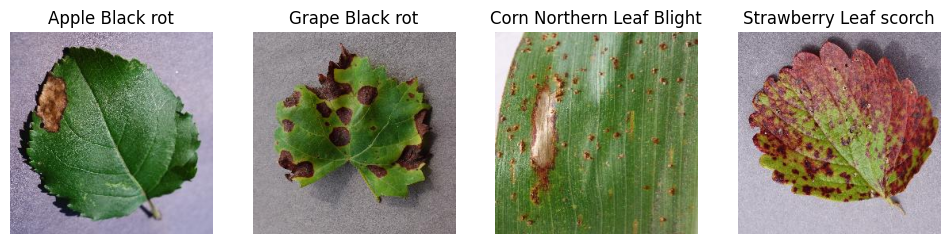
\includegraphics[width=15cm]{../images/example_images_of_plantvillage.png}
    \caption{Example images of PlantVillage}
    \label{fig:example_images_of_plantvillage}
    \end{center}
\end{figure}

This dataset does not provide a split for a test test. Therefore, the splitting was carried out by myself using 80/% training, 10\% validation and test data respectively. The stratifying ensures, that the class distribution is the same over all sets, which can be seen in Figure {fig:class_distribution_of_plantvillage}.  
The PlantVillage dataset has 38 different classes including different plants and diseases. 

\begin{figure}[H]
    \begin{center}
    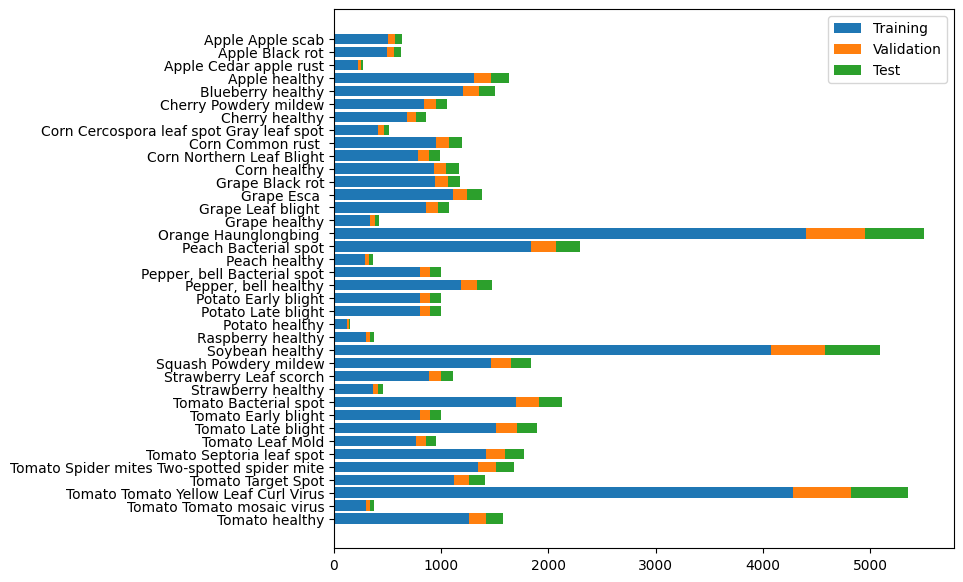
\includegraphics[width=15cm]{../images/class_distribution_of_plantvillage.png}
    \caption{Class distribution of PlantVillage}
    \label{fig:class_distribution_of_plantvillage}
    \end{center}
\end{figure}

\section{Models}
